\documentclass[letter,10pt,oneside]{article}
 
\usepackage{amsfonts}
\usepackage{amsmath}
\DeclareMathOperator*{\amax}{arg\,max}
\DeclareMathOperator*{\amin}{arg\,min}
\usepackage{amssymb}
\usepackage{mathabx}
\usepackage{dsfont}

\usepackage{epsf}
\usepackage{epsfig}
\usepackage{graphicx}
%\usepackage{wrapfig}
%\usepackage{subfig}

\usepackage{setspace}
\usepackage{geometry}
\usepackage{fancyhdr}

\usepackage{hyperref}
\hypersetup{
    colorlinks,
    citecolor=blue,
    filecolor=blue,
    linkcolor=blue,
    urlcolor=blue
}

\usepackage[latin2]{inputenc}
\usepackage{lmodern} % ez eltu"nteti a raszteressget s mg jk is a betu"k
\usepackage{t1enc}


\usepackage[usenames]{color}
%\usepackage[colorlinks]{hyperref}
%\usepackage{showkeys}

%\onehalfspacing
\usepackage{indentfirst}
%\frenchspacing

\usepackage{listings}
\definecolor{mygreen}{rgb}{0,0.6,0}
\definecolor{mygray}{rgb}{0.5,0.5,0.5}
\definecolor{mymauve}{rgb}{0.58,0,0.82}

\lstset{ %
  backgroundcolor=\color{white},   % choose the background color; you must add \usepackage{color} or \usepackage{xcolor}; should come as last argument
  basicstyle=\footnotesize,        % the size of the fonts that are used for the code
  breakatwhitespace=false,         % sets if automatic breaks should only happen at whitespace
  breaklines=true,                 % sets automatic line breaking
  captionpos=b,                    % sets the caption-position to bottom
  commentstyle=\color{mygreen},    % comment style
  deletekeywords={...},            % if you want to delete keywords from the given language
  escapeinside={\%*}{*)},          % if you want to add LaTeX within your code
  extendedchars=true,              % lets you use non-ASCII characters; for 8-bits encodings only, does not work with UTF-8
  frame=single,	                   % adds a frame around the code
  keepspaces=true,                 % keeps spaces in text, useful for keeping indentation of code (possibly needs columns=flexible)
  keywordstyle=\color{blue},       % keyword style
  language=python,                 % the language of the code
  morekeywords={*,...},           % if you want to add more keywords to the set
  numbers=left,                    % where to put the line-numbers; possible values are (none, left, right)
  numbersep=5pt,                   % how far the line-numbers are from the code
  numberstyle=\tiny\color{mygray}, % the style that is used for the line-numbers
  rulecolor=\color{black},         % if not set, the frame-color may be changed on line-breaks within not-black text (e.g. comments (green here))
  showspaces=false,                % show spaces everywhere adding particular underscores; it overrides 'showstringspaces'
  showstringspaces=false,          % underline spaces within strings only
  showtabs=false,                  % show tabs within strings adding particular underscores
  stepnumber=1,                    % the step between two line-numbers. If it's 1, each line will be numbered
  stringstyle=\color{mymauve},     % string literal style
  tabsize=4,	                   % sets default tabsize to 2 spaces
  title=\lstname                   % show the filename of files included with \lstinputlisting; also try caption instead of title
}

\geometry{left=2.5cm,right=2.5cm,top=3.0cm,bottom=2.5cm}

\pagestyle{fancy}
\lhead{ }
\chead{ }
\rhead{\thepage}

\lfoot{ }
\cfoot{ }
\rfoot{P\'{e}ter K\'{o}m\'{a}r, Totient Inc., 2019}


\renewcommand{\headrulewidth}{0.4pt}
\renewcommand{\footrulewidth}{0.0pt}

\newcommand{\bel}{\begin{equation}}
\newcommand{\eel}{\end{equation}}
\newcommand{\be}{\begin{equation*}}
\newcommand{\ee}{\end{equation*}}

\newcommand{\bal}{\begin{eqnarray}}
\newcommand{\eal}{\end{eqnarray}}
\newcommand{\ba}{\begin{eqnarray*}}
\newcommand{\ea}{\end{eqnarray*}}

\newcommand{\ket}[1]{| #1 \rangle}
\newcommand{\Ket}[1]{\left| #1 \right\rangle}
\newcommand{\bra}[1]{\langle #1 |}
\newcommand{\Bra}[1]{\left\langle #1 \right|}

\newcommand{\no}{\noindent}

\newcommand{\ev}[1]{\langle #1 \rangle}
\newcommand{\Ev}[1]{\left\langle #1 \right\rangle}
\newcommand{\+}{^\dagger}
\newcommand{\s}{^\odot}
\newcommand{\T}{^\top}
\newcommand{\LL}{\mathcal{L}}
\newcommand{\PP}{\mathcal{P}}

\newcommand{\low}{\text{low}}
\newcommand{\high}{\text{high}}
\newcommand{\MLE}{\text{MLE}}

\newcommand{\refeq}[1]{Eq. \ref{#1}}
\newcommand{\reffig}[1]{Fig. \ref{#1}}

\newcommand{\blue}[1]{{\color{blue} #1}}


%\numberwithin{equation}{section}
%\numberwithin{figure}{section}
%\numberwithin{table}{section}

\author{P\'{e}ter K\'{o}m\'{a}r (Totient Inc.)}
\title{Development notes for \texttt{deldenoiser}}
\date{\today}


\begin{document}


\thispagestyle{empty}
\maketitle

\no {\bf One sentence summary: } This note contains the statistical, algorithmic and implementation details for the DNA-encoded library denoising tool ``deldenoiser''.

\tableofcontents

\newpage


\section{Background}


\subsection{DNA-encoded libraries}

A DNA-encoded library (DEL) consist of a collection of DNA-tagged ligand molecules synthesized according to a prescribed design. Each DNA sequence corresponds uniquely to one of many ligands constructed combinatorially from a predefined set of building blocks. (See \reffig{fig:DEL_overview}a.)

DEL synthesis is typically performed in split-pool cycles, each of which consists of different parallel reactions where a unique tag and building block is attached to participating molecules. The library complexity is increasing geometrically with the number of synthesis cycles, enabling the simultaneous synthesis of many different compounds, given enough initial material. (See \reffig{fig:DEL_overview}b.)

High-affinity ligands are found by a binding essay, where anchored target proteins localize strongly binding molecules while weakly binding ones are eliminated. Sequencing the tags of selected molecules provides a quantitative measure of their relative fitness, from which the protein-ligand association constants can be determined. (See \reffig{fig:DEL_overview}c.)

\begin{figure}[h]
  \centering
  \includegraphics[width=0.5\textwidth]{figs/DEL_overview.pdf}
  \caption{
    \label{fig:DEL_overview}
    DNA-encoded library. {\bf a.} Design and library of uniquely tagged ligand compounds. {\bf b.} Split-pool cycles of synthesis creates combinatorial variety. {\bf c.} Binding assay selects high-affinity ligands.
  }
\end{figure}


\subsection{Truncated compounds}

The chemical reactions employed in constructing the ligands often fail to convert all participating molecules to the desired product. Truncates, molecules of the remaining initial compound and of unwanted side-products, contaminate the library. Since DNA tags are attached to molecules based on the reaction conditions they were subjected to, but irrespective of their true chemical composition, these incomplete ligands masquerade as full-cycle compounds in the sequencing result.

Restricting the design to rely only on high-yield reactions is overly limiting. Here we present a method capable of suppressing the noise due to the most common type of truncation: incomplete conversions of a reactant to the corresponding product. Relying on knowing the yields of reactions, involving mock scaffolds and selected building blocks, which are typically performed prior to full-scale DEL synthesis, we deconvolve the sequencing read counts, and estimate the fitness of truncated and full-cycle products.


\section{Model}

We present the ``null block'' model, which accounts for the contamination of DELs due to remnants of intermediate products. This model is over-complete and requires regularization to avoid overfitting. We show how an L1-type regularization results in a computationally efficient inference algorithm.

\subsection{Notation}

\begin{itemize}
  \item $c \in \{1,2,\ldots C\}$ is the index of synthesis cycles.

  \item $r = (r_1, r_2, \ldots r_C)$ is the reaction index combination of any one full-cycle product, where $r_c \in \{1,2,\ldots R_c\}$ is the index of reaction in cycle $c$.
  
  \item $s = (s_1, s_2, \ldots s_C)$, where $s_c \in \{0,1\}$, is the success vector that indicates which synthesis steps were successful.
  
  \item $q = (q_1, q_2, \ldots q_C)$ is the ligand composition vector, where $q_c \in \{0\}\cup \{1,2,\ldots R_c\}$ indexes the building block that was attached in cycle $c$, and 0 stands for missing building block or ``null block''. It can be expressed with the success vector $s$ and the reaction index vector $r$ as $q = s \odot r$, where $\odot$ stands for elementwise multiplication.

  \item $\mathcal{F} = \{q\;:\; (\forall c: q_c \neq 0)\}$ is the set of full-cycle ligands, the ones that do not contain any null blocks.

  \item $\mathcal{T} = \{q\;:\; (\exists c: q_c = 0)\}$ is the set of truncated ligands, the ones which have at least one null block.
  
  \item $Y_{c, r_c}$ is the yield of reaction $r_c$ in cycle $c$ (assumed to depend solely on the identity of a building block participating in a given reaction), a value between 0 and 1.

  \item $N_r$ is the number of sequencing reads of the tag associated with the reaction index combination $r$. We will use $N^\text{pre}_r$ and $N^\text{post}_r$ to indicate the read counts from the sequencing experiment done before and after the DEL selection steps, respectively.

  \item $\lambda_r$ is the expected number of reads, an unknown, which is a function of other model parameters. We will use $\lambda_r^\text{pre}$ and $\lambda_r^\text{post}$ to denote expected read counts obtained before and after selection.

  \item $C_\text{sel}$ is the number of selection cycles.

  \item $[\text{P}]$ is the concentration of the target protein during binding assays, measured in $\text{mol}/\text{l}$.

  \item $K_q$ is the association constant of the ligand $q$, measured in $(\text{mol}/\text{l})^{-1}$.

  \item $F_q$ is the relative fitness of ligand $q$, a positive number that is proportional to the overall survival chance $S_q$ of ligand $q$.

  \item $S_q$ is the probability of ligand $q$ surviving all $C_\text{sel}$ selection cycles.

  \item $[\text{L}_{r, q}]$ is the concentration of molecules with DNA tags associated with reaction indexes $r$ and ligand composition $q$.

  \item $\gamma$ is the dispersion parameter of the dispersed-Poisson distribution. Values $\gamma > 1$ indicate that the variance of the read count is $\gamma$ times larger than its mean. Choosing $\gamma = 1$ is identical to assuming a regular Poisson noise on the number of reads.

\end{itemize}

\subsection{Data}

We assume that the following pieces of data are known.
\begin{itemize}
  \item Per-cycle reaction yields $Y_{c, r_c} \in [0, 1]$ for all $c$ and $r_c$.
  \item Pre-selection read counts, $N^\text{pre}_r \in\{0, 1, 2, \ldots\}$ for all $r$, obtained by sequencing the tags before selection.
  \item Post-selection read counts, $N^\text{post}_r\in\{0, 1, 2, \ldots\}$ for all $r$, obtained by sequencing the tags after selection.
\end{itemize}


\subsection{Pre-selection sequencing}

Sequencing the library before the binding assay provides information about potential imbalances due to differences in nucleotide content of the DNA tags. Each tag $r$ has an associated Poisson intensity $\lambda^\text{pre}_r$, i.e. the expected number of sequencing reads. We model the observed $N^\text{pre}_r$ with a dispersed Poisson distribution,
\bel
  \label{eq:dispersed-Poisson}
  P(N^\text{pre}_r = N \;|\; \lambda^\text{pre}_r = \lambda) = Z(\lambda, \gamma) \frac{(\lambda / \gamma)^{N/\gamma}}{\Gamma(N/\gamma + 1)},
\eel
defined on non-negative integer $N$, where $\Gamma$ is the gamma function, and the normalization constant is $Z(\lambda, \gamma) \approx \exp(-\lambda / \gamma) / \gamma$. The dispersion parameter $\gamma$ controls the variance $\text{Var}(N) \approx \gamma \cdot \mathbb{E}(N) = \gamma \lambda$. For $\gamma = 1$, this formula reverts back to the standard Poisson distribution. 

Ideally, the total number of reads is large enough that the maximum likelihood result, $\hat\lambda_r = N_r$ (which is independent of $\gamma$) provides a good estimate. If, however, individual $r$ index combinations get few reads due to low sequencing depth, then we need to lower the model complexity. Instead of assuming that all $\lambda_r^{\text{pre}}$ are independent, we model them as a product of $C$ independent factors, one for each cycle. 
\bel
  \label{eq:b-factors}
  \lambda_r^\text{pre} = N^\text{pre}_\text{tot}\cdot b_{1, r_1}\cdot b_{2, r_2}\cdot \ldots b_{C, r_C} = N^\text{pre}_\text{tot}\prod _c b_{c, r_c}
\eel
Instead of $\prod_c R_c$ number of $\{\lambda_r^\text{pre}\}$ parameter, this model has $\sum_c R_c$ number of $\{b_{c, r_c}\}$ parameters, enabling inference even at low sequencing depths. The maximum likelihood estimates of $b$ (see derivation in Appendix \ref{app:pre-selection-MLE-result}),
\bel
\label{eq:b-factor-MLE}
  \hat b_{c, r_c} = \frac{1}{N^\text{pre}_\text{tot}}\sum_{r': r'_c = r_c} N^\text{pre}_{r'},
\eel
can be used to compute an estimates of the Poisson intensities,
\bel
  \hat \lambda^\text{pre}_r = N^\text{pre}_\text{tot}\prod _c \hat b_{c, r_c}.
\eel
We assume that the same imbalances are in play during the post-selection sequencing, and we use the normalized pre-selection imbalance estimates $\hat \lambda^\text{pre}_r / N^\text{pre}_\text{tot}$ to correct sequencing imbalance in the post-selection data.


\subsection{Synthesis}

During cycle $c$ of the synthesis a piece of DNA tag, indexed by $r_c$, gets appended and the corresponding synthesis reaction takes place. If the synthesis reaction succeeds ($s_c = 1$) the intended building block $q_c = r_c$ is attached. But if truncation happens ($s_c = 0$), we denote it by setting $q_c = 0$. After $C$ cycles of synthesis, each DNA tag labels potentially $2^C$ different compounds (each associated with a different success vector $s$). Their relative amounts can be expressed as a product of yields: $Y_{c, r_c}$ if $s_c = 1$, or $(1 - Y_{c, r_c})$ if $s_c = 0$. The concentration of ligand $\text{L}_{r,q}$ right after synthesis and before selection can be written as 
\bel
  [\text{L}_{r,q=s\odot r}]_\text{pre} = [\text{L}_{r,q=r}]_\text{ideal} \underbrace{\prod_c (Y_{c, r_c})^{s_c} (1 - Y_{c, r_c})^{(1 - s_c)}}_{=:J_{r, s}},
\eel
where $[\text{L}_{r,q=r}]_\text{ideal}$ is the concentration of ligand $r$ if all yields were 100\%, and we defined $J_{r,s}$ to be the relative fraction of ligands $s\odot r$ among all molecules tagged with $r$. Note that we assume that only those $\text{L}_{r,q}$ molecules are present for which $q = \text{sgn}(q)\odot r$, and the concentration of all other molecules is zero.


\subsection{Selection}

During the binding assay, each ligand L settles in a thermodynamic equilibrium with the protein P and the ligand-protein complex L:P,
\bel
\label{eq:L-P-reaction}
  \text{L:P} \quad \rightleftharpoons \quad \text{L} \; + \; \text{P}
\eel
The concentration of the complex in equilibrium $[\text{L:P}]_\text{eq}$ is a function of the initial ligand concentration $[\text{L}]_\text{init}$, the protein concentration $[\text{P}]$ and the association constant $K$, (see derivation in Appendix \ref{app:lignad-protein-complex-concentration})
\bel
\label{eq:L:P_concentration}
  [\text{L:P}]_\text{eq} = [\text{L}]_\text{init} \left(1 + \frac{1}{K[\text{P}]}\right)^{-1},
\eel
where we assumed that the initial concentration of the protein is large enough that it is not depleted significantly by the totality of \emph{all} ligand-protein reactions.

After the equilibrium is reached, the remaining free ligands are washed away, the complexes get converted back to free ligands and the next selection cycle starts. After $C_\text{sel}$ selection cycles the remaining ligand concentration is 
\bel
  [\text{L}_{r,q}]_\text{post} = [\text{L}_{r,q}]_\text{pre} \underbrace{\left(1 + \frac{1}{K_q[\text{P}]}\right)^{-C_\text{sel}}}_{=:S_q},
\eel
where $[\text{L}_{r,q}]_\text{pre}$ is the ligand concentration before selection, and we defined $S_q$ to be the survival chance of ligand $q$. Note that we assume that only the ligand composition $q$ determines the association constant, and the DNA tag $r$ plays no role here.

\subsection{Post-selection sequencing}

After synthesis and selection, the remaining molecules go through sequencing  identical to the pre-selection one. We assume that a dispersed Poisson distribution explains the read counts $N^\text{post}_r$, 
\bel
  \label{eq:dispersered-Poisson_post}
  P(N^\text{post}_r = N \;|\; \lambda^\text{post}_r = \lambda) = Z(\lambda, \gamma) \frac{(\lambda / \gamma)^{N/\gamma}}{\Gamma(N/\gamma + 1)},
\eel
where the expected mean of each count is proportional to the amount of ligands with the corresponding tag $r$,
\bal
  \lambda_r^\text{post} &=& N_\text{tot}^\text{post} k^\text{post} \eta_r A^\text{post}\sum_q [\text{L}_{r,q}]_\text{post}   \\
  &=& N_\text{tot}^\text{post} k^\text{post} \eta_r A^\text{post}\sum_s [\text{L}_{r,q = s\odot r}]_\text{post} \\
  \label{eq:lambda_r_post}
  &=& N_\text{tot}^\text{post} k^\text{post} \eta_r A^\text{post}[\text{L}_{r,r}]_\text{ideal} \sum_s  J_{r,s} S_{q=s\odot r},
\eal
where the $A^\text{post}$ factor accounts for the increase of amount of DNA due to PCR amplification as well as any other planned reduction of the total amount of DNA, (and for calibration purposes, explained in section \ref{sec:postprocessing}, $A^\text{pre}$ and $A^\text{post}$ are assumed to be known). The factor $\eta_r$ is the tag-dependent sequencing bias, whose value is unimportant, and $k^\text{post}$ is an unknown normalization factor making sure that $\sum_r\lambda_r^\text{post} = N_\text{tot}^\text{post}$.

The same equation for the pre-selection expected read counts would look like
\bel
\label{eq:lambda_r_pre}
  \lambda_r^\text{pre} = N_\text{tot}^\text{pre} k^\text{pre} \eta_r A^\text{pre}[\text{L}_{r,r}]_\text{ideal},
\eel
because $\sum_s J_{r,s} = 1$. We compare \refeq{eq:lambda_r_post} and \refeq{eq:lambda_r_pre} and use the estimates $\hat \lambda_r^\text{pre}$ to express $\lambda_r^\text{post}$ as
\bal
\label{eq:lambda_post}
  \lambda_r^\text{post} &=& \sum_s \left(\frac{N_\text{tot}^\text{post}}{N_\text{tot}^\text{pre}}\hat\lambda_r^\text{pre} J_{r,s}\right) \left(\frac{k^\text{post}A^\text{post}}{k^\text{pre}A^\text{pre}} S_{q=s\odot r}\right) \\
  &=& \sum_q \underbrace{\left(\frac{N_\text{tot}^\text{post}}{N_\text{tot}^\text{pre}}\hat\lambda_r^\text{pre} \cdot [\text{sgn}(q)\odot r = q]\cdot J_{r,s=\text{sgn}(q)}\right)}_{=:X_{r,q}} \underbrace{\left(\frac{k^\text{post}A^\text{post}}{k^\text{pre}A^\text{pre}} S_{q}\right)}_{=:F_q},
\eal
where $[\text{sgn}(q)\odot r = q] = 1$, if $\text{sgn}(q)\odot r = q$, and $0$ otherwise, and $\text{sgn}(q)$ is the result of the sign function applied to each element of the $q$ vector. The matrix $X$ can be computed directly from the data since $\hat \lambda_r^\text{pre}$ can be estimated from the pre-selection read counts and the matrix $J$ is a function of the per-cycle reaction yields, which we assumed to be known. We package the unknown factors, $k^\text{pre}$, $k^\text{post}$ and $S_q$ into the  variables $F_q$, the ``fitness'' of each ligand $q$. Since $F_q$ is proportional to $S_q$, which is a monotonically increasing function of $K_q$, estimates of $F_q$ can be used to rank ligands by affinity.


\subsection{Regularization}

We can summarize the generative model for the post-selection read counts $N^\text{post}$, defined by \refeq{eq:dispersered-Poisson_post} and \refeq{eq:lambda_post}, as
\bel
  P(N_r^\text{post}\;|\;\lambda_r^\text{post}) = \text{disperesed-Poisson}(N_r^\text{post}\;|\;\lambda_r^\text{post}, \gamma), \qquad \text{where }\quad  \lambda_r^\text{post} = \sum_q X_{r,q} F_q.
\eel
This is a generalized linear model with dispersed Poisson noise and identity link function. A simple model in itself. The difficulty is caused by the fact that the number of parameters $\{F_q\}_{q \in \mathcal{F} \cup \mathcal{T}}$, is larger than the number of data points $\{N^\text{post}_r\}_{r \in \mathcal{F}}$,
\bel
  |\mathcal{F} \cup \mathcal{T}| = \prod_c (R_c + 1) \quad >\quad  \prod_c R_c = |\mathcal{F}|.
\eel
Consequently, to enable inference, we need to regularize the model. To do this, we choose a practical prior distribution for the $F_q \;(>0)$  parameters, 
\bel
\label{eq:prior}
  P(F) = \prod_q P(F_q) = \prod_q \alpha \exp(-\alpha F_q),
\eel
which promotes sparse solutions, i.e. a large number of ligands will be estimated to have zero fitness. The sparsity promoted by this choice of prior reflects our expectation that many ligands will have negligible affinity. The regularization strength, $\alpha$, is the inverse of the a priori expected value of $F_q$. While we expect the true $F_q$ values to vary across many orders of magnitudes due to large differences in affinity, this spread is centered around 1. This suggest that the theoretical optimal value of $\alpha$ is 1. (See Appendix \ref{app:best_alpha} for more detailed argument.)


\subsection{Inference of fitness of truncates}

With the exponential prior, the log posterior of the fitness vector, $\log P(F\;|\;N^\text{post})$, can be written as
\bal
  \log P(\{F_q\}\;|\;\{N_r^\text{post} = N_r\}) &=& \log \Big(P(N^\text{post}\;|\; F) \,P(F)\Big)  + \text{const.} \\
  &=& \log\left(\Big[\prod_r P(N_r^\text{post} = N_r\;|\;\lambda_r^\text{post}\Big]\Big[\prod_q P(F_q)\Big]\right) + \text{const.}\\
  &=& \sum_r \log\left(\text{disperesed-Poisson}(N_r\;|\;\lambda_r^\text{post}, \gamma)\right) + \sum_q \log \Big(\alpha \exp(-\alpha F_q)\Big) + \text{const.}\\
  &=& \sum_r \left[-\frac{1}{\gamma} \sum_q X_{r,q}F_q + \frac{N_r}{\gamma}\log\left(\sum_q X_{r,q}F_q\right)\right] + \sum_q (-\alpha) F_q + \text{const.}
  \label{eq:log_posterior_full_F}
\eal
where $\text{const.}$ denotes terms independent of $F$. 

Although, with the regularization terms, this function admits to direct maximization with respect to the unknown $\{F_q\}$ parameters, we can improve the robustness of the inference algorithm by averaging over the fitness parameters of the full-cycle products, $\{F_q\}_{q\in \mathcal{F}}$ (see derivation in Appendix \ref{app:LP-of-truncates}, yielding the log posterior of the fitness of the truncates $\{F_q\}_{q\in\mathcal{T}}$,
\bal
  \log P(\{F_q\}_{q\in\mathcal{T}}\;|\;N^\text{post}) &=& \log\left(\intop\!dF_{q\in \mathcal{F}}\, P(F\;|\;N^\text{post})\right) \\ 
  &=& \sum_{r\in\mathcal{F}}\left[\frac{\alpha}{X_{r,r}}B_r + \log\Gamma\!\left(\frac{N_r}{\gamma} + 1,\; \Big(\frac{\alpha}{X_{r,r}} + \frac{1}{\gamma}\Big) B_r\right)\right] - \alpha \sum_{q\in\mathcal{T}} F_q,
  \label{eq:log_posterior_truncated_F}
\eal
where $B_r = \sum_{q \in \mathcal{T}} X_{r,q}F_q$ is the Poisson intensity contributions of all truncates to the read count of tag $r$, and $\Gamma(s, x)$ is the incomplete gamma function defined by the integral, $\Gamma(s, x) = \intop_x^\infty\!dt\, t^{s-1} e^{-t}$, which can be efficiently evaluated with e.g. python's \texttt{scipy.special.gammaincc} function. With the fitness parameters of the full-cycle products averaged over, the number of parameters that need optimizing is greatly reduced.

Although the fitness coefficients of the truncates cannot be estimated independently because they couple via the sum making up $B_r$ terms, their interdependence is weak because discrepancies between $N_r$ and $B_r$ are smoothly explained away by the potential presence of of high-fitness full-cycle products. This motivates the following coordinate descent strategy for optimizing $\{F_q\}_{q\in\mathcal{T}}$, starting from the all-zero vector.
\begin{enumerate}
  \item Fix all $F_q$ except $q = q_{(0)} := (0,0,0,\ldots 0)$, and directly maximize the log-posterior (\refeq{eq:log_posterior_truncated_F}) as a function of the single variable, $F_{q_{(0)}}$. This yields an estimate for the fitness of the truncate $q_{(0)}$.
  \item Fix all $F_q$ values, except for $q$ where only one element is non-zero, and find the optimal values for their corresponding $F_q$ parameters one-by-one.
  \item Fix all $F_q$ values, except for $q$s with one more non-zero element than previously, and repeat the optimization for them, one at a time.
  \item Keep increasing the number of non-zero $q$ elements, up to $C-1$, and perform the optimization for each $F_q$ for the selected $q$. Once done, we will have computed all $\hat F_q$ estimates for the truncates $q \in \mathcal{T}$.
\end{enumerate}
Performing these steps once realizes a single iteration of coordinate descent. We run multiple iterations until all intensity contributions, $B_r$, change less than a predefined tolerance threshold. This strategy converges to the global maximum of the log posterior because the cost function, $f(F) =  - \log P(\{F_q\}_{q \in \mathcal{T}}\;|\; N^\text{post})$ is a convex function of $F$. (See proof in Appendix \ref{app:convexity}.)


\subsection{Inference of fitness of full-cycle products}

With estimates obtained for the fitness of truncates $\{\hat F_q\}_{q\in\mathcal{T}}$, we can go back to the log posterior of $F$ (\refeq{eq:log_posterior_full_F}) and estimate the fitness of full-cycle products $\{F_r\}_{r\in\mathcal{F}}$. This can be done independently from each other by maximizing their individual log posteriors, 
\bel
\label{eq:full-cycle-LP}
  \log P(F_r\;|\; N_r, \{F_q\}_{q\in\mathcal{T}}) = -\frac{1}{\gamma}(B_r + X_{r,r}F_r) + \frac{N_r}{\gamma}\log (B_r + X_{r,r}F_r) - \alpha F_r,
\eel
where $B_r = \sum_{q\in \mathcal{T}} X_{r,q} \hat F_q$. The posterior mode, expectation value and variance of $F_r$, are
\bal
  \label{eq:F_r_mode}
  (F_r)^\ast &=& \text{max}\left(0,\;\frac{N_r}{X_{r,r} + \gamma \alpha} - \frac{B_r}{X_{r,r}}\right), \\
  \label{eq:F_r_ev}
  \mathbb{E}(F_r) &=& \frac{G_1}{X_{r,r} + \gamma \alpha} - \frac{B_r}{X_{r,r}}, \\
  \label{eq:F_r_var}
  \text{Var}(F_r) &=& \frac{G_2 - (G_1)^2}{(X_{r,r} + \gamma \alpha)^2},
\eal
where
\bal
  G_1 &=& \frac{\gamma\cdot\Gamma(n_r + 1,\, x_r)}{\Gamma(n_r, \, x_r)} \\
  G_2 &=& \frac{\gamma^2\cdot\Gamma(n_r + 2,\, x_r)}{\Gamma(n_r, \, x_r)},
\eal
where $n_r = N_r / \gamma + 1$ and $x_r = B_r (1/\gamma + \alpha/X_{r,r})$.


\subsection{Breakdown of post-selection read counts}
With the estimates $\hat F_q$ for all ligands $q$, we can break down the post-selection read counts by different $s$ success vectors. Given the observed count $N_r^\text{post} = N_r$, and the $\hat F_q$ estimates (using either the modes $(F_r)^\ast$ or the expectation values $\mathbb{E}(F_r)$ for full-cycle products), the distribution of the counts belonging to different $s$ success vectors is distributed according to a multinomial distribution,
\bel
  P(\{N_{r,s}\}_s\;|\;N_r, \{\hat F_q\}) = \text{Multinomial}(\{N_{r,s}\}\;|\;N_r, \{p_{r,s}\}), \qquad \text{where }\; p_{r,s} = \frac{X_{r,q=s\odot r} \hat F_{q=s\odot r}}{\sum_{s'}X_{r,q=s'\odot r} \hat F_{q=s'\odot r}},
\eel
and the expected values of the sub-read count $N_{r,s}$ is $\mathbb{E}(N_{r,s}) = N_r p_{r,s}$.


\section{Postprocessing}
\label{sec:postprocessing}

The inference algorithm presented in the previous section estimates the fitness $F_q$ of each ligand $q$. Here, we explain that with additional calibration information, we can compute the corresponding $S_q$ survival rates, and $K_q$ association constants.

\subsection{Need for survival rate calibration}

While we trust our assumption that the number of reads are proportional to the concentration of the corresponding DNA tag $r$, we do not know the value of the proportionality constant. In other words, the two experiment-specific factors $k^\text{pre}$ and $k^\text{post}$, which convert molecule concentrations $[\text{L}_{r,q}]$ into read counts $N_r$, are unknown. This poses the problem that, while we can estimate the fitness $F_q$ of each ligand, we have no handle on their survival rate $S_q$, and association constant $K_q$, because (see \refeq{eq:lambda_post})
\bel
  F_q = \frac{k^\text{post}A^\text{post}}{k^\text{pre}A^\text{pre}} S_q = \frac{k^\text{post}A^\text{post}}{k^\text{pre}A^\text{pre}} \left(1 + \frac{1}{K_q[\text{P}]}\right)^{-C_\text{sel}},
\eel
where the $A$ factors are assumed to be known, but the $k$ factors are not.

Due to the definition of survival chance, which prevents it from being larger than 1, we can put a lower bound on the proportionality factor $\frac{k^\text{post} A^\text{post}}{k^\text{pre} A^\text{pre}} \geq \text{max}\{F_q\}$, but since it's possible that even the ligand with the highest affinity has a survival chance much smaller than 1, this lower bound can be far from the actual value.

To get accurate survival rate estimates, we need additional data. The simplest of all would be using a special ``calibration ligand'', a known binder with known true survival rate $S^\ast$. With its estimated fitness coefficient $F^\ast$, we can compute the proportionality factor as
\bel
  \frac{k^\text{post}A^\text{post}}{k^\text{pre}A^\text{pre}} = \frac{F^\ast}{S^\ast},
\eel
which then can be used to compute $S_q$ and $K_q$ for all other $q$ molecules
\bel
  \hat S_q = \frac{S^\ast}{F^\ast}\cdot \hat F_q,\qquad \hat K_q = \frac{1}{[\text{P}]}\frac{(\hat S_q)^{1/C_\text{sel}}}{1 - (\hat S_q)^{1/C_\text{sel}}}.
\eel
Unfortunately, we cannot expect such a ``calibration ligand'' to be universally available, because the target protein P will change from screen to screen. Below, we present two alternative ways of calibration.

\subsection{Measuring the total amount of DNA}
This calibration method relies on measuring the amount of DNA before and after selection, and hinges on the assumption that $[\text{L}_{r,r}]_\text{ideal}$ in uniform across all $r$.

The total amount of DNA before and after selection can be expressed as
\bal
  n_\text{pre} &=& \sum_r \sum_s [\text{L}_{r,q=s\odot r}]_\text{pre} = \sum_r [\text{L}_{r,q=r}]_\text{ideal} \underbrace{\sum_{s}J_{r,s}}_{=1}, \\
  n_\text{post} &=& \sum_r \sum_s [\text{L}_{r,q=s\odot r}]_\text{post} = \sum_r [\text{L}_{r,q=r}]_\text{ideal} \sum_s J_{r,s} S_{q = s\odot r},
\eal
where $S_q$ can also be expressed with the corresponding fitness $F_q$,
\bel
  S_q = \frac{k^\text{pre}A^\text{pre}}{k^\text{post}A^\text{post}} F_q.
\eel
With the assumption that $[\text{L}_{r,r}]_\text{ideal}$ is the same for all $r$, the ratio of the amounts of DNA before and after selection, can be written as
\bel
  \frac{n_\text{post}}{n_\text{pre}} = \frac{k^\text{pre}A^\text{pre}}{k^\text{post}A^\text{post}} \frac{\sum_r \sum_s J_{r,s} F_{s\odot r}}{\sum_r 1},
\eel
which allows us to express the estimates $S_q$ with the $\hat F_q$ estimates as
\bel
  \hat S_q = \frac{k^\text{pre}A^\text{pre}}{k^\text{post}A^\text{post}} \hat F_q = \frac{n_\text{post}}{n_\text{pre}} \frac{\sum_r 1}{\sum_r \sum_s J_{r,s} \hat F_{s\odot r}} \;\hat F_q.
\eel
This method relies on measuring the pre- and post-selection DNA amounts accurately and works only if it is justified to assume that the effects participating in tag creation (e.g. DNA ligation) do not discriminate different $r$ tags, and therefore we can assume that $[\text{L}_{r,r}]_\text{ideal}$ is the same for all $r$.

\subsection{DNA spike-in}
The second method of calibration uses the read counts of uniquely distinguishable sequences of DNA (e.g. Illumina's PhiX sequencing control) mixed in just before sequencing. It can be used if we can accurately control the amplification factors $A^\text{post}$ and $A^\text{pre}$ and the amount of added DNA.

Let $\phi$ denote the added DNA, $\lambda_\phi$ its expected read count and $[\phi]$ its concentration. Assuming that $\phi$ is added after PCR amplification ($A_\phi = 1$), we can express its expected read counts in the two sequencing experiments (pre- and post-selection) as
\bal
  \lambda_\phi^\text{pre} &=& N_\text{tot}^\text{pre} k^\text{pre} \eta_\phi [\phi]_\text{pre}, \\
  \lambda_\phi^\text{post} &=& N_\text{tot}^\text{post} k^\text{post} \eta_\phi [\phi]_\text{post},
\eal
where $\eta_\phi$ is the sequencing efficiency of $\phi$, whose value is unimportant. The expected read counts of $\phi$ can be estimated by the observed ones, $\hat \lambda_\phi = N_\phi$, for both experiments, allowing us to express the ratio of the normalization constants as
\bel
  \frac{k^\text{pre}}{k^\text{post}} = \frac{N_\phi^\text{pre} / N_\text{tot}^\text{pre}}{N_\phi^\text{post} / N_\text{tot}^\text{post}}\frac{[\phi]_\text{post}}{[\phi]_\text{pre}},
\eel
which can be used to compute $\hat S_q$ from $\hat F_q$ as
\bel
  \hat S_q = \frac{N_\phi^\text{pre} / N_\text{tot}^\text{pre}}{N_\phi^\text{post} / N_\text{tot}^\text{post}}\frac{[\phi]_\text{post}}{[\phi]_\text{pre}}\frac{A^\text{pre}}{A^\text{post}}\;\hat F_q.
\eel
This method relies on the accurate knowledge of the $A$ factors and the $[\phi]$ concentrations, but does not require any additional assumptions.




\begin{appendix}


\section{Computational details}
We explain how some of the mathematical formulas can be evaluated efficiently.

\subsection{Operations with matrix $X$}
The $X = [[X_{r,q}]_{q \in \mathcal{F}\cup \mathcal{T}}]_{r\in\mathcal{F}}$ matrix, defined by 
\be
  X_{r,q} = \frac{N_\text{tot}^\text{post}}{N_\text{tot}^\text{pre}}\hat\lambda_r^\text{pre} \cdot [\text{sgn}(q)\odot r = q]\cdot J_{r,s=\text{sgn}(q)}
\ee
is very sparse. It contains at most $2^C$ non-zero elements in each row, because it is constructed from the elements of the $J$ matrix, which has only $2^C$ columns. Therefore it is more efficient to store only these elements in a smaller matrix $\tilde X = [[\tilde X_{r,s}]_{s \in \{0,1\}^C}]_{r\in\mathcal{F}}$, where
\be
  \tilde X_{r,s} = \frac{N_\text{tot}^\text{post}}{N_\text{tot}^\text{pre}}\hat\lambda_r^\text{pre} J_{r,s}.
\ee
Using this form, the matrix product between $X$ and $F$, i.e. $\sum_q X_{r,q} F_{q}$, can be computed in two steps:
\begin{enumerate}
  \item Compute the $\tilde F = [[\tilde F_{r,s}]_{s \in \{0,1\}^C}]_{r\in\mathcal{F}}$ matrix from the $F = [F_q]_{q\in\mathcal{F}\cup \mathcal{T}}$ vector, such that
  \be
    \tilde F_{r,s} = F_{q=r\odot s}.
  \ee

  \item Evaluate the sum over the columns of the elementwise product of $\tilde X$ and $\tilde F$,
  \be
    \sum_q X_{r,q} F_{q} = \sum_s \tilde X_{r,s} \tilde F_{r,s}.
  \ee
\end{enumerate}
This requires the same number of multiplications as a direct sparse-matrix implementation, but avoids doing unnecessary bookkeeping.

\subsection{Computing $\log \Gamma(s, x)$}
The upper incomplete gamma function,
\bel
  \Gamma(s, x) = \intop_x^\infty \! dt\, t^{s-1} e^{-t}
\eel
can be computed efficiently with python's \texttt{scipy.special.gammaincc(s, x)} function call, which computes the \emph{normalized} upper incomplete function, $\Gamma(s,x) / \Gamma(s)$. We make two small adjustments to this solution to obtain accurate result of its logarithm and speed up computation.
\begin{enumerate}
  \item Since we are interested in the logarithm of $\Gamma(s, x)$, we need to avoid numerical underflow. We achieve this by checking if \texttt{scipy.special.gammaincc} returns 0, and if so, we evaluate the first few terms of the asymptotic series of $\log \Gamma(s,x)$ instead.
  \be
    \log \Gamma(s,x) \approx -x + (s-1) \log(x) + \log\left(1 + \frac{s-1}{x}\right),
  \ee
  which is accurate if $x > s$, which is exactly the case when we expect $\Gamma(s,x)$ to underflow.

  \item During the DEL denoising problem the first argument of $\Gamma(s, x)$, $s$, is often equal to 1, (this happens for each term where the read count $N_r$ is zero). For these cases, we use the identity,
  \be
    \log\Gamma(1,x) = -x,
  \ee
  to speed up computation.
\end{enumerate}

\section{Derivations}
In this section we provide the mathematical derivations of the results used throughout the document.

\subsection{Maximum likelihood estimate of $\lambda^\text{pre}$}
\label{app:pre-selection-MLE-result}
The log likelihood of the per-cycle factors of the pre-selection Poisson intensity is defined by the dispersed Poisson distribution from \refeq{eq:dispersed-Poisson}. It can be written as
\ba
  \log P(\{N_r^\text{pre}\}\;|\;\{b_{c,r_c}\}) 
  &=& \sum_r \log P(N_r^\text{pre}\;|\;\{b_{c,r_c}\}) \\
  &=& \sum_r \left[\log Z(\lambda_r^\text{pre}, \gamma) + \frac{N_r}{\gamma}\log\left(\frac{\lambda_r^\text{pre}}{\gamma}\right) - \log\Gamma\left(\frac{N_r^\text{pre}}{\gamma} + 1\right)\right] \\
  &=& \sum_r \left[-\log \gamma - \frac{\lambda_r^\text{pre}}{\gamma} + \frac{N_r^\text{pre}}{\gamma} \log\left(\frac{\lambda_r^\text{pre}}{\gamma}\right) - \log\Gamma\left(\frac{N_r^\text{pre}}{\gamma} + 1\right)\right].
\ea
where we used the approximation $Z(\lambda, \gamma)\approx \exp(-\lambda / \gamma) / \gamma$, which is accurate if $\gamma$ is close to 1, or if $\lambda$ is larger than 10. Using the definition of the $b$ factors from \refeq{eq:b-factors}, we can express the above log likelihood as
\ba
   \log P(\{N_r^\text{pre}\}\;|\;\{b_{c,r_c}\}) 
  &=& \sum_r\left[-\frac{N_\text{tot}^\text{pre}}{\gamma} \prod_c b_{c, r_c} + \frac{N_r^\text{pre}}{\gamma}\sum_c \log b_{c, r_c}\right] + \text{const.}
\ea
where $\text{const.}$ stands for terms independent of the $b$ factors. Without loss of generality, we assume that the $b$ factors are normalized for each cycle separately,
\be
  \sum_{r_c} b_{c, r_c} = 1,
\ee
and use the method of Lagrange-multipliers to incorporate this constraint to the maximization of the log likelihood. This is done by taking the derivative of $\log P + \sum_c \Lambda_c(1 - \sum_{r_c} b_{c,r_c})$ with respect to $b_{c,r_c}$, and solving them for zero, and determining the values of the Lagrange multipliers $\{\Lambda_c\}$ using the normalization constraints.
\ba
  0 
  &=& \frac{\partial}{\partial b_{c, r_c}}\left(\log P(\{N_{r'}^\text{pre}\}\;|\;\{b_{c',{r'}_{c'}}\})  + \sum_{c'} \Lambda_{c'}\Big(1 - \sum_{{r'}_c'} b_{c',{r'}_{c'}}\Big)\right) 
  \\ 
  &=& -\frac{N_\text{tot}^\text{pre}}{\gamma}\frac{\partial}{\partial b_{c, r_c}} \left(\sum_{r'} \prod_{c'} b_{c',{r'}_{c'}}\right) + \sum_{r'} \frac{N_{r'}^\text{pre}}{\gamma}\sum_{c'} \frac{\partial}{\partial b_{c, r_c}} \Big(\log b_{c',{r'}_{c'}}\Big) - \sum_{c'} \Lambda_{c'} \sum_{r'} \frac{\partial}{\partial b_{c, r_c}} \Big(b_{c',{r'}_{c'}}\Big)
\ea
We evaluate the three derivative terms separately. First,
\be
  \frac{\partial}{\partial b_{c, r_c}} \left(\sum_{r'} \prod_{c'} b_{c',{r'}_{c'}}\right) = \frac{\partial}{\partial b_{c, r_c}} \left(\prod_{c'} \sum_{{r'}_{c'}}  b_{c',{r'}_{c'}}\right) = 0
\ee
because $\sum_{{r}_{c}}  b_{c,{r}_{c}} = 1$ is constant. The second the third terms are non-zero only if $c = c'$ and $r_c = {r'}_{c'}$, which we indicate with the Kronecker delta symbols $\delta_{c,c'} \delta_{r_c, {r'}_c}$:
\ba
  \frac{\partial}{\partial b_{c, r_c}} \Big(\log b_{c',{r'}_{c'}}\Big) &=& \delta_{c,c'} \delta_{r_c, r'_c} \frac{1}{b_{c, r_c}} \\
  \frac{\partial}{\partial b_{c, r_c}} \Big(b_{c',{r'}_{c'}}\Big) &=& \delta_{c,c'} \delta_{r_c, {r'}_c}.
\ea
Plugging these back into the sum yields
\ba
  0 
  &=& \frac{1}{\gamma} \sum_{r'} N_{r'}^\text{pre} \sum_{c'} \delta_{c,c'}\delta_{r_c, r'_c} \frac{1}{b_{c,r_c}} - \sum_{c'} \Lambda_{c'} \delta_{c,c'} \sum_{r'} \delta_{r_c, {r'}_c}
  \\
  &=& \frac{1}{\gamma}\frac{1}{b_{c, r_c}} \sum_{r'}\delta_{r_c,{r'}_c} N_{r'}^\text{pre} - \Lambda_c \sum_{r'} \delta_{r_c, {r'}_c}
  \\
  &=&  \frac{1}{\gamma}\frac{1}{b_{c, r_c}} \sum_{r': r'_c = r_c}N_{r'}^\text{pre} - \Lambda_c \sum_{r': {r'}_c = r_c} 1
\ea 
Solving for $b_{c, r_c}$ yield the maximum likelihood estimate
\be
  \hat b_{c, r_c} = \frac{1}{\gamma \Lambda_c \sum_{r':{r'}_c=r_c} 1} \sum_{r':{r'}_c = r_c} N_r^\text{pre},
\ee
where the $\Lambda_c$ constants can be found using the constraint,
\be
  1 = \sum_{r_c}\hat b_{c, r_c} = \frac{1}{\gamma \Lambda_c \sum_{r':{r'}_c=r_c} 1} \underbrace{\sum_{r_c}\sum_{r':{r'}_c = r_c} N_{r'}^\text{pre}}_{\sum_{r'} N_{r'}^\text{pre} = N_\text{tot}^\text{pre}},
\ee
giving
\be
  \hat b_{c, r_c} = \frac{1}{N_\text{tot}^\text{pre}} \sum_{r':{r'}_c = r_c} N_{r'}^\text{pre},
\ee
which is \refeq{eq:b-factor-MLE}.


\subsection{Equilibrium concentration of ligand-protein complex}
\label{app:lignad-protein-complex-concentration}

The thermodynamic equilibrium between free ligands and ligand-protein complexes is described by \refeq{eq:L-P-reaction},
\be
  \text{L:P} \quad \rightleftharpoons\quad  \text{L} \quad +\quad  \text{P}.
\ee
At the beginning of each selection cycle the protein concentration is $[\text{P}]_\text{init}$, the free ligand concentration is $[\text{L}]_\text{init}$ and the concentration of L:P complex is zero. The equilibrium concentrations are related to each other due to conservation of ligand and protein molecules,
\bal
\label{eq:app:LP=L}
  {}[\text{L:P}]_\text{eq} + [\text{L}]_\text{eq} &=& [\text{L}]_\text{init}, \\
  {}[\text{L:P}]_\text{eq} + [\text{P}]_\text{eq} &=& [\text{P}]_\text{init},
\eal
and they are also connected by the association constant of the ligand-protein complex $K$, via the law of mass action,
\bel
\label{eq:app:K}
  K = \frac{[\text{L:P}]_\text{eq}}{[\text{L}]_\text{eq}[\text{P}]_\text{eq}}.
\eel
We use the assumption that the the protein concentration is high enough that settling in equilibrium does not change it significantly, i.e. $[\text{P}]_\text{eq} \approx [\text{P}]_\text{init} =: [\text{P}]$. Combining \refeq{eq:app:LP=L} and \refeq{eq:app:K} yields
\be
  K [\text{L}]_\text{eq}[\text{P}] = [\text{L}]_\text{init} - [\text{L}]_\text{eq},
\ee
which can be solved for $[\text{L}]_\text{eq}$, giving
\be
  [\text{L}]_\text{eq} = \frac{[\text{L}]_\text{init}}{1 + K[\text{P}]},
\ee
which, substituted back to \refeq{eq:app:LP=L} yields the equilibrium concentration of the complex,
\be
  {}[\text{L:P}]_\text{eq} = [\text{L}]_\text{init} - [\text{L}]_\text{eq} = [\text{L}]_\text{init}\left(1 - \frac{1}{1 + K[\text{P}]}\right) = [\text{L}]_\text{init} \left(1 + \frac{1}{K[\text{P}]}\right)^{-1},
\ee
which is \refeq{eq:L:P_concentration}.

\subsection{Theoretical optimal value for $\alpha$}
\label{app:best_alpha}
The regularization strength $\alpha$ governs how strongly the model favors sparse $F_q$ solutions. Realistically, tuning $\alpha$ is going to require  running the inference algorithm with different $\alpha$ choices and choosing the one that produces the desired results. Here, we present theoretical consideration why setting $\alpha = 1$ is a good starting point.

Let us start with the expression of $\lambda_r^\text{post}$ from \refeq{eq:dispersered-Poisson_post},
\be
  \lambda_r^\text{post} = \sum_q X_{r,q} F_q,
\ee
and let us require that the a priori expected value of the sum of $\lambda_r^\text{post}$ is equal to $N_\text{tot}^\text{post}$,
\bal
  N_\text{tot}^\text{post} 
  &=& \mathbb{E}\Big(\sum_r \lambda_r^\text{post}\Big)
  \nonumber\\
  &=& \sum_r  \mathbb{E}(\lambda_r^\text{post})
  \nonumber\\
  \label{eq:app:sumXEF}
  &=& \sum_r \sum_q X_{r,q} \mathbb{E}(F_q).
\eal
Here $\mathbb{E}(F_q)$ is the a priori expectation value of the fitness coefficients. Since, in \refeq{eq:prior}, we assumed them the be distributed according to an exponential distribution with parameter $\alpha$, their expectation value is
\be
  \mathbb{E}(F_q) = \frac{1}{\alpha}.
\ee
Substituting this back to \refeq{eq:app:sumXEF} yields
\be
  N_\text{tot}^\text{post}  = \sum_r \sum_q X_{r,q} \frac{1}{\alpha},
\ee
which allows us to write $\alpha$ as
\ba
  \alpha 
  &=& \frac{1}{N_\text{tot}^\text{post}} \sum_r \sum_q X_{r,q} 
  \\
  &=& \sum_r \sum_q \frac{\hat \lambda_r^\text{pre}}{N_\text{tot}^\text{pre}} [\text{sgn}(q)\odot r = q] J_{r, s=\text{sgn}(q)} 
  \\
  &=& \sum_r \frac{\hat \lambda_r^\text{pre}}{N_\text{tot}^\text{pre}} \underbrace{\sum_s J_{r,s}}_{=1}
  \\
  &=& \frac{1}{N_\text{tot}^\text{pre}} \underbrace{\sum_r \hat \lambda_r^\text{pre}}_{=N_\text{tot}^\text{pre}} = 1.
\ea

This shows that if we use the total post-selection read counts to set the prior of $F_q$, the optimal choice is $\alpha = 1$.

\subsection{Averaging over full-cycle fitness parameters}
\label{app:LP-of-truncates}
Taking the exponential of \refeq{eq:log_posterior_full_F} gives the posterior of the fitness vector $F$, up to a constant factor
\ba
  P(F\;|\;N^\text{post} = N) 
  &\propto& \exp\left(\sum_r\left[-\frac{1}{\gamma}\sum_q X_{r,q} F_q + \frac{N_r}{\gamma}\log\Big(\sum_q X_{r,q} F_q\Big)\right] - \alpha\sum_q F_q\right) \\
  &=& \left[\prod_r \exp\Big(-\frac{1}{\gamma}\sum_q X_{r,q} F_q\Big) \left(\sum_q X_{r,q}F_q\right)^{N_r / \gamma}\right]\left[\prod_q e^{-\alpha F_q}\right]
\ea
We make use of an important property of the $X$ matrix, namely that in any column corresponding to full-cycle compounds, $q \in \mathcal{F}$, only one $X_{r,q}$ element is non-zero, the one for which $r = q$, i.e. 
\be
  X_{q,r} = \delta_{q,r} X_{r,r},\qquad \forall q \in \mathcal{F}.
\ee
This reflects that, according to the null-block model, full-cycle products are created only if no truncations happen. This allows us to separate the full cycle products from the truncates in the equation of the posterior and average over them one-by-one.
\be
  \sum_q X_{r,q} F_q = \sum_{q\in \mathcal{F}\cup \mathcal{T}} X_{r,q} F_q = \sum_{q\in\mathcal{F}}X_{r,q}F_q + \sum_{q\in\mathcal{T}}X_{r,q}F_q = X_{r,r}F_r + \underbrace{\sum_{q\in\mathcal{T}}X_{r,q}F_q}_{=:B_r},
\ee
where $B_r$ is the Poisson intensity due to the truncated molecules. Substituting this to the formula for the posterior yield
\ba
  P(F\;|\;N^\text{post}) 
  &\propto& \Bigg[\prod_{r\in\mathcal{F}} \underbrace{\exp\Big(-\frac{1}{\gamma}(X_{r,r}F_r  + B_r)\Big) \left(X_{r,r}F_r + B_r\right)^{N_r / \gamma} \exp(-\alpha F_r)}_{=:I_r(F_r)}\Bigg] \left[\prod_{q \in \mathcal{T}}\exp(-\alpha F_q)\right].
\ea
Averaging over the fitness of the full-cycle products $\{F_r\}_{r\in\mathcal{F}}$ requires us to evaluate the following integral
\bel
\label{eq:app:likelihood-of-truncates}
  P(\{F_q\}_{q\in\mathcal{T}}\;|\;N^\text{post}) = \intop\! dF_{q\in\mathcal{F}} \, P(F\;|\;N^\text{post}) = \left[\prod_{r\in \mathcal{F}} \intop_0^\infty\!dF_r\, I_r(F_r)\right]\left[\prod_{q \in \mathcal{T}}\exp(-\alpha F_q)\right],
\eel
where the single-variable integrals $\intop_0^\infty\!dF_r I_r(F_r)$ can be evaluated separately. For simplicity, we suppress the $r$ indexes on $X$, $B$, and $N$, and use the dummy variable $f$ in place of $F_r$ and write the integral as
\ba
  \mathcal{I}_r = \intop_0^\infty \!df I_r(f) 
  &=& \intop_0^\infty \!df e^{-\alpha f} e^{-\frac{1}{\gamma}(Xf + B)} \left(\frac{1}{\gamma}(Xf + B)\right)^{N/\gamma}.
\ea
We introduce a new integration variable,
\be
  y = \frac{1}{\gamma}(Xf + B),\qquad f = \frac{\gamma y - B}{X},\qquad df = \frac{\gamma}{X} dy, 
\ee
which allows us to write the integral as
\ba
  \mathcal{I}_r 
  &=& 
  \intop_{B / \gamma}^\infty \!dy\, \frac{\gamma}{X} \,e^{\frac{\alpha B}{X}} \,e^{-\left(\frac{\gamma\alpha}{X} + 1\right)y} \,y^{N / \gamma} 
  \\
  &=& 
  \frac{\gamma}{X} e^{\frac{\alpha B}{X}} \intop_{B/\gamma}^\infty \!dy\, y^{N/\gamma} \, e^{-\left(\frac{\gamma\alpha}{X} + 1\right)y}.
\ea
We change the integration variable once again to
\be
  z = \left(\frac{\gamma\alpha}{X}+1\right)y,\qquad y = \frac{z}{\frac{\gamma\alpha}{X}+1},\qquad dy = \frac{dz}{\frac{\gamma\alpha}{X}+1},
\ee
giving
\ba
  \mathcal{I}_r 
  &=& 
  \frac{\gamma}{X} e^{\frac{\alpha B}{X}} \intop_{\left(\frac{\gamma\alpha}{X} + 1\right)\frac{B}{\gamma}}^\infty\!dz\, \frac{1}{\frac{\gamma \alpha}{X} + 1}\, e^{-z} \frac{z^{N/\gamma}}{\left(\frac{\gamma\alpha}{X} + 1\right)^{N/\gamma}} 
  \\
  &=& 
  \frac{\gamma}{X} e^{\frac{\alpha B}{X}} \frac{1}{\left(\frac{\gamma\alpha}{X} + 1\right)^{N/\gamma + 1}} \underbrace{\intop_{\left(\frac{\gamma\alpha}{X} + 1\right)\frac{B}{\gamma}}^\infty\!dz\,e^{-z}\, z^{N/\gamma}}_{\Gamma\left(\frac{N}{\gamma} + 1,\, \Big(\frac{\gamma\alpha}{X} + 1\Big)\frac{B}{\gamma}\right)},
\ea
where $\Gamma(s, x)$ is the upper incomplete gamma function. Substituting this result to \refeq{eq:app:likelihood-of-truncates} allows us to write the log of  posterior of the truncates as
\ba
  \log P(\{F_q\}_{q\in\mathcal{T}} \;|\; N^\text{post}) 
  &=&
  \log\left(\Big[\prod_{r\in \mathcal{F}} \mathcal{I}_r\Big]\Big[\prod_{q \in \mathcal{T}}\exp(-\alpha F_q)\Big]\right) + \text{const.}
  \\
  &=& 
  \sum_{r\in\mathcal{F}} \log \mathcal{I}_r - \alpha\sum_{q\in\mathcal{T}} F_q + \text{const.}
  \\
  &=&
  \sum_r \left[\frac{\alpha B_r}{X_{r,r}} + \log\Gamma\!\left(\frac{N_r}{\gamma} + 1,\, \Big(\frac{\alpha}{X_{r,r}} + \frac{1}{\gamma}\Big)B_r\right)\right] - \alpha\sum_{q\in\mathcal{T}} F_q + \text{const.}
\ea
yielding \refeq{eq:log_posterior_truncated_F}, where $B_r = \sum_{q\in\mathcal{T}}X_{r,q} F_q$. 

We note that, since the incomplete gamma function can be evaluated efficiently, finding the optimal values of the fitness of the truncates $\{F_q\}_{q\in\mathcal{T}}$ via maximizing this $\log P$ is more efficient than maximizing the original log posterior over the much larger number of \emph{all} fitness coefficients $\{F_q\}_{q\in\mathcal{F}\cup\mathcal{T}}$.

We were able to average over the fitness coefficients of the full-cycle products in closed form because of the specific choice of the dispersed Poisson distribution. If we used negative binomial distribution, which is more widely used, instead, we would not have been able to evaluate the $\mathcal{I}_r$ in closed form, preventing us to improve the efficiency of the inference algorithm.

\subsection{Proof of convexity of log posterior}
\label{app:convexity}
\refeq{eq:log_posterior_truncated_F} provides the formula for the log posterior of the fitness coefficient of the truncates $F_q$. Here we show that its negative, i.e. $-\log P$, is a convex function of $F_q$, therefore it has a single local minimum, which is also the global minimum.

First, since $-\alpha \sum_{q\in\mathcal{T}} F_q$ is a linear function of $F$, we can disregard it, as it does not affect the convexity of the sum. Second, since $\alpha B_r /X_{r,r}$ are linear functions of $F$, we can disregard them too. This leaves us with having to show that each of the 
\be
  - \log\Gamma\!\left(\frac{N_r}{\gamma} + 1,\, \Big(\frac{\alpha}{X_{r,r}} + \frac{1}{\gamma}\Big)B_r\right)
\ee
terms are convex in $F$. Since the expression $\Big(\frac{\alpha}{X_{r,r}} + \frac{1}{\gamma}\Big)B_r$ is a linear functions of $F$, and the composition of a convex function and a linear function is convex, it is enough to show that $-\log \Gamma(s, x)$ is convex in its second argument, $x$, for all $s \geq 1$ integers.

Here, we show that the second derivative of $-\log \Gamma(s, x)$ is non-negative for all $x>0$ values if $s\geq 1$, thereby proving that the function is convex. The second derivative can be written as
\be
  \left(\frac{\partial}{\partial x}\right)^2 \Big[-\log \Gamma(s, x)\Big] = \left(\frac{\partial}{\partial x}\right) \left[\frac{x^{s-1} e^{-x}}{\Gamma(s,x)}\right] = - \frac{x^{s-1} e^{-x}}{(\Gamma(s, x))^2} (-x^{s-1} e^{-x}) + \frac{-x^{s-1}e^{-x} + (s-1)x^{s-2} e^{-x}}{\Gamma(s,x)}.
\ee
Since both $\Gamma(s, x)$ and $x^{s-1} e^{-x}$ are positive, it is enough to show that
\be
  f(x) = x^{s-1} e^{-x} + \Gamma(s,x) \left(-1 + \frac{s-1}{x}\right)
\ee
is non-negative. For $x \leq s-1$ this is trivially true, because then even the $(-1 + (s-1)/x)$ factor is non-negative. For the $x > s-1$ case, we use the following upper bound for $\Gamma(s,x)$, (which can be constructed from continued fraction expression of the incomplete gamma function (which converges for all non-negative $s$ integers),
\be
  \Gamma(s, x) =  \frac{x^s e^{-x}}{1 + x - s + \epsilon} \leq \frac{x^s e^{-x}}{1 + x - s},
\ee
where $\epsilon$ is a positive correction. Because $(-1 + (s-1)/x)$ is negative, with this upper bound, we can establish the following \emph{lower} bound of $f(x)$
\ba
  f(x) \;=\; x^{s-1} e^{-x} - \Gamma(s,x) \left(1 - \frac{s-1}{x}\right) &\geq & x^{s-1} e^{-x} - \frac{x^s e^{-x}}{1 + x - s} \left(1 - \frac{s-1}{x}\right) \\
  &=& x^{s-1}e^{-x} \left[1 - \frac{x}{1 + x-s}\Big(1 - \frac{s-1}{x}\Big)\right] \\
  &=& x^{s-1}e^{-x}\left[1 - \frac{1}{1 - \frac{s-1}{x}}\Big(1 - \frac{s-1}{x}\Big) \right] \\
  &=& 0.
\ea
This finishes the proof of the convexity of $-\log P$.

\subsection{Estimates of fitness of full-cycle products}
\label{app:full-cycle-fitness}
From the expression of the log posterior of the fitness of full-cycle products, \refeq{eq:full-cycle-LP}, 
\be
  \log P(F_r\;|\;N_r, \{F_q\}_{q\in \mathcal{T}}) = -\frac{1}{\gamma}(B_r + X_{r,r}F_r) + \frac{N_r}{\gamma}\log(B_r + X_{r,r} F_r) - \alpha F_r
\ee
we derive the mode, expectation value and variance of $F_r$.

Requiring that the first derivative to be zero yield the mode,
  \ba
    \frac{\partial}{\partial F_r} \log P = -\frac{X_{r,r}}{\gamma} + \frac{N_r X_{r,r}}{\gamma(B_r + X_{r,r}F_r)} - \alpha &=& 0  \\
    \frac{N_r}{\gamma}\frac{X_{r,r}}{B_r + X_{r,r}F_r} &=& \alpha + \frac{X_{r,r}}{\gamma} \\
    N_r &=& \left(\frac{\alpha\gamma}{X_{r,r}} + 1\right) B_r + (\alpha\gamma + X_{r,r})F_r \\
    F_r &=& \frac{N_r}{\alpha \gamma + X_{r,r}} - \frac{B_r}{X_{r,r}}.
  \ea
  Considering that $F_r$ must be non-negative, results in \refeq{eq:F_r_mode}.  
  
The expectation value and the variance of $F_r$ are
\ba
  \mathbb{E}(F_r) &=& \frac{\intop_0^\infty \! df \, f\, P(f\;|\;N_r, B_r)}{\intop_0^\infty \! df \, P(f\;|\;N_r, B_r)} \;=:\; \frac{Z_1}{Z_0}\\
  \text{Var}(F_r) &=& \frac{\intop_0^\infty \! df \, f^2\, P(f\;|\;N_r, B_r)}{\intop_0^\infty \! df \, P(f\;|\;N_r, B_r)} -  (\mathbb{E}(F_r))^2  \;=:\; \frac{Z_2}{Z_0} - \left(\frac{Z_1}{Z_0}\right)^2,
\ea
where $P(F_r\;|\;N_r, B_r) = \exp(\log P(F_r\;|\;N_r, B_r))$, is the \emph{unnormalized} posterior.
We evaluate $Z_0$, $Z_1$ and $Z_2$ below (where we drop the $r$ indexes for the sake of simplicity)
\begin{itemize}
  \item $Z_0$ 
  \ba
    Z_0 &=& \intop_0^\infty \! df \, e^{-\frac{1}{\gamma}(B + Xf)} \cdot (B + Xf)^{N/\gamma} \cdot e^{-\alpha f}
    \\
    &=& \intop_{B/\gamma}^\infty \! dz\; \frac{\gamma}{X} \cdot e^{-z}\cdot z^{N/\gamma} \cdot e^{-\frac{\alpha}{X}(\gamma z - f)}
    \\
    &=& \frac{\gamma}{X} e^{\frac{\alpha B}{X}} \gamma^{N/\gamma} \intop_{\left(\frac{1}{\gamma} + \frac{\alpha}{X}\right)B}^\infty \!dy\, \frac{1}{1 + \frac{\alpha \gamma}{X}} \left(\frac{y}{1 + \frac{\alpha \gamma}{X}}\right)^{N/\gamma} \cdot e^{-y} 
    \\
    &=& \frac{1}{X}\cdot e^\frac{\alpha B}{X} \left(\frac{1}{\gamma} + \frac{\alpha}{X}\right)^{-(N/\gamma + 1)} \cdot \Gamma\!\left(\frac{N}{\gamma} + 1,\,\Big(\frac{1}{\gamma} + \frac{\alpha}{X}\Big)B\right)
  \ea
  where we introduced two new integration variables $z = (B + Xf) / \gamma$, and $y = (1 + \alpha\gamma / X)z$.

  \item $Z_1$
  \ba
    Z_1 &=& \intop_0^\infty \! df \, f\cdot e^{-\frac{1}{\gamma}(B + Xf)} \cdot (B + Xf)^{N/\gamma} \cdot e^{-\alpha f}
    \\
    &=& 
    \intop_{B/\gamma}^\infty \! dz\; \frac{\gamma}{X} \cdot \frac{\gamma z - B}{X}\cdot e^{-z}\cdot z^{N/\gamma} \cdot e^{-\frac{\alpha}{X}(\gamma z - f)}
    \\
    &=& 
    \frac{\gamma}{X^2} e^\frac{\alpha B}{X} 
    \Bigg[
      \gamma^{N/\gamma + 1} 
      \hspace{-0.3cm}
      \underbrace{
        \intop_{B/\gamma}^\infty\!dz \, z^{N/\gamma + 1} \cdot e^{-\left(1 + \frac{\alpha\gamma}{X}\right)z}
      }_{
        \left(1 + \frac{\alpha\gamma}{X}\right)^{-(N/\gamma + 2)} \Gamma\left(\frac{N}{\gamma} + 2,\, \left(\frac{1}{\gamma} + \frac{\alpha}{X}\right)B\right)
      } 
      -\quad  
      B\gamma^{N/\gamma}
      \hspace{-0.5cm}
      \underbrace{
        \intop_{B/\gamma}^\infty\!dz \, z^{N/\gamma} \cdot e^{-\left(1 + \frac{\alpha\gamma}{X}\right)z}
      }_{
        \left(1 + \frac{\alpha\gamma}{X}\right)^{-(N/\gamma + 1)} \Gamma\left(\frac{N}{\gamma} + 1,\, \left(\frac{1}{\gamma} + \frac{\alpha}{X}\right)B\right)
      }
    \hspace{-0.3cm}
    \Bigg]
    \\
    &=&
    \frac{1}{X^2} e^{\frac{\alpha B}{X}}\left(\frac{1}{\gamma} + \frac{\alpha}{X}\right)^{-(N/\gamma + 1)} \left[\frac{\Gamma\!\left(\frac{N}{\gamma} + 2,\,\big(\frac{1}{\gamma} + \frac{\alpha}{X}\big)B\right)}{\frac{1}{\gamma} + \frac{\alpha}{X}} - B\cdot\Gamma\!\left(\frac{N}{\gamma} + 1,\,\Big(\frac{1}{\gamma} + \frac{\alpha}{X}\Big)B\right)\right] ,
  \ea
  where, in the second line, we used the same change of variables as before $z = (B+Xf) / \gamma$

  \item $Z_2$
  \ba
    Z_2 &=& \intop_0^\infty \! df \, f^2\cdot e^{-\frac{1}{\gamma}(B + Xf)} \cdot (B + Xf)^{N/\gamma} \cdot e^{-\alpha f}
    \\
    &=& 
    \intop_{B/\gamma}^\infty \! dz\; \frac{\gamma}{X} \cdot \frac{(\gamma z - B)^2}{X^2}\cdot e^{-z}\cdot z^{N/\gamma} \cdot e^{-\frac{\alpha}{X}(\gamma z - f)}
    \\
    &=& \frac{1}{X^3}\gamma^{N/\gamma + 1} e^\frac{\alpha B}{X}
    \Bigg[
      \gamma^2 
        \intop_{B/\gamma}^\infty\!dz\, z^{N/\gamma + 2} e^{-\left(1 + \frac{\alpha\gamma}{X}\right)z}
      - 2\gamma B
        \intop_{B/\gamma}^\infty\!dz\, z^{N/\gamma + 1} e^{-\left(1 + \frac{\alpha\gamma}{X}\right)z} 
        \\
        &&\hspace{2.7cm}
      + B^2 
        \intop_{B/\gamma}^\infty\!dz\, z^{N/\gamma} e^{-\left(1 + \frac{\alpha\gamma}{X}\right)z}
    \Bigg]
    \\
    &=& 
    \frac{1}{X^3}e^\frac{\alpha B}{X} \left(\frac{1}{\gamma} + \frac{\alpha}{X}\right)^{-(N/\Gamma + 1)}\left[\frac{\Gamma\!\left(\frac{N}{\gamma} + 3, x\right)}{\left(\frac{1}{\gamma} + \frac{\alpha}{X}\right)^2} -2B \frac{\Gamma\!\left(\frac{N}{\gamma} + 2, x\right)}{\frac{1}{\gamma} + \frac{\alpha}{X}} + B^2 \Gamma\!\left(\frac{N}{\gamma} + 1, x\right)\right],
  \ea
  where we use the shorthand $x = \left(\frac{1}{\gamma} + \frac{\alpha}{X}\right)B$.
\end{itemize}
Substituting these results in place of $Z_0, Z_1, Z_2$ in the definition of the expectation value and the variance, we get
\ba
  \mathbb{E}(F_r) &=& \frac{Z_1}{Z_0} = \underbrace{\frac{\gamma\cdot\Gamma\!\left(\frac{N}{\gamma}+2,\,x\right)}{\Gamma\!\left(\frac{N}{\gamma}+1,\,x\right)}}_{=:G_1}\frac{1}{X + \alpha \gamma} - \frac{B}{X}
  \\
  \text{Var}(F_r) &=& \frac{Z_2}{Z_0} - \left(\frac{Z_1}{Z_0}\right)^2 = \underbrace{\frac{\gamma^2\cdot\Gamma\!\left(\frac{N}{\gamma}+3,\,x\right)}{\Gamma\!\left(\frac{N}{\gamma}+1,\,x\right)}}_{=:G_2}\frac{1}{(X + \alpha \gamma)^2} - \frac{(G_1)^2}{(X + \alpha\gamma)^2}
\ea
which, after re-introducing the indexes to $B_r$, $N_r$ and $x_r = \left(\frac{1}{\gamma} + \frac{\alpha}{X_{r,r}}\right)\!B_r$, become \refeq{eq:F_r_ev} and \refeq{eq:F_r_var}.
\end{appendix}







\end{document}
